\documentclass{article}
\usepackage{graphicx}
\usepackage{amsmath}
\usepackage{amssymb}
\usepackage{amsfonts}
\usepackage{tikz}
\usetikzlibrary{positioning, arrows.meta}

\title{Strategy State Transition Diagram with Conditional Probabilities}
\author{Geoffrey Wang}
\date{August 2024}

\begin{document}

\maketitle

\section*{Introduction}

This document provides an explanation of the strategy state transition diagram for the Hawk-Dove game with mixed strategies. The diagram visualizes the conditions under which strategies transition from one to another and the conditional probabilities associated with these transitions.

\section*{Strategy Transition Conditions and Probabilities}

In the Q-learning model, the conditions for strategy transitions can be summarized as follows:

\begin{itemize}
    \item \textbf{Hawk to Dove}:
    \begin{itemize}
        \item \textbf{Condition}: If the Q-value of Dove is higher than that of Hawk, there is a higher probability of transitioning from Hawk to Dove.
        \item \textbf{Probability}: Dependent on the exploration rate $\epsilon$ and the relative size of the Q-values.
    \end{itemize}
    
    \item \textbf{Dove to Hawk}:
    \begin{itemize}
        \item \textbf{Condition}: If the Q-value of Hawk is higher than that of Dove, there is a higher probability of transitioning from Dove to Hawk.
        \item \textbf{Probability}: Same as above.
    \end{itemize}
    
    \item \textbf{Mixed to Hawk or Dove}:
    \begin{itemize}
        \item \textbf{Condition}: If the mixed strategy selects Hawk or Dove and performs well in a match, the mixed strategy will tend to focus on the strategy that performed better.
        \item \textbf{Probability}: The direction of the transition is determined by the ratio of Q-values.
    \end{itemize}
\end{itemize}

\section*{State Transition Diagram with Conditional Probabilities}

The following diagram represents the strategy state transitions along with the conditions and probabilities:

\begin{figure}[h!]
    \centering
    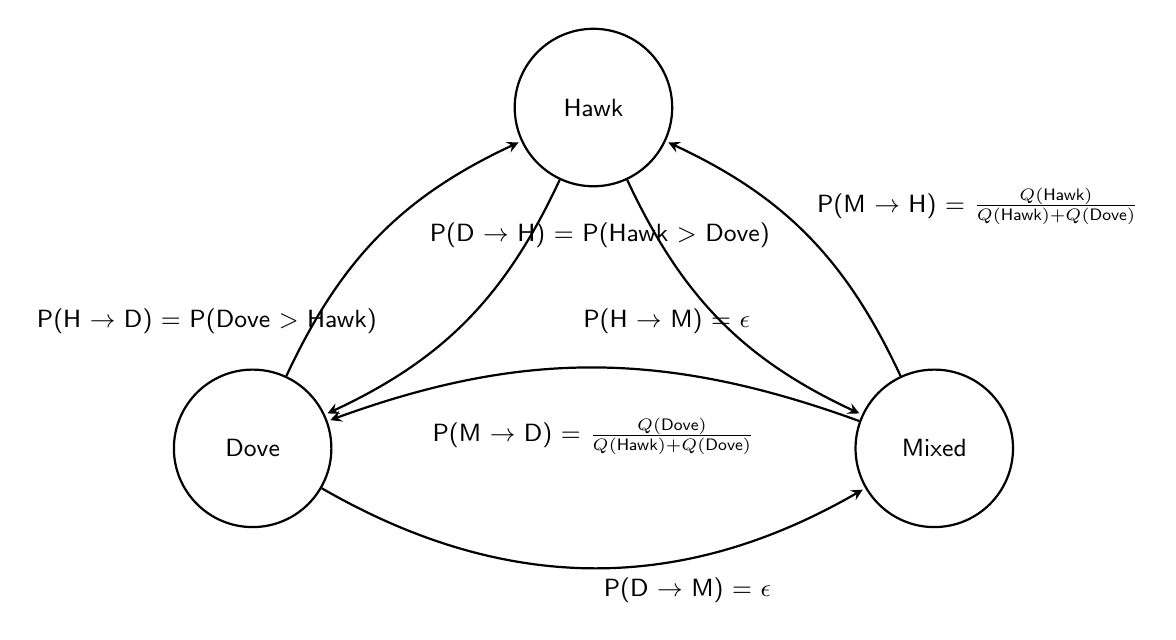
\begin{tikzpicture}[->,>=stealth,shorten >=1pt,auto,node distance=4cm, thick,
      main/.style={circle,draw,minimum size=2cm, font=\sffamily\small}]

      \node[main] (H) {Hawk};
      \node[main] (D) [below left of=H, xshift=-1.5cm, yshift=-1.5cm] {Dove};
      \node[main] (M) [below right of=H, xshift=1.5cm, yshift=-1.5cm] {Mixed};

      \path[every node/.style={font=\sffamily\small}]
        (H) edge [bend left=20] node [left, xshift=-1cm] {P(H $\rightarrow$ D) = P(Dove $>$ Hawk)} (D)
            edge [bend right=20] node [left, xshift=0.5cm] {P(H $\rightarrow$ M) = $\epsilon$} (M)
        (D) edge [bend left=20] node [right, xshift=0.5cm] {P(D $\rightarrow$ H) = P(Hawk $>$ Dove)} (H)
            edge [bend right=30] node [below right] {P(D $\rightarrow$ M) = $\epsilon$} (M)
        (M) edge [bend right=20] node [above right] {P(M $\rightarrow$ H) = $\frac{Q(\text{Hawk})}{Q(\text{Hawk}) + Q(\text{Dove})}$} (H)
            edge [bend right=20] node [below, yshift=-0.5cm] {P(M $\rightarrow$ D) = $\frac{Q(\text{Dove})}{Q(\text{Hawk}) + Q(\text{Dove})}$} (D);
    \end{tikzpicture}
    \caption{Strategy State Transition Diagram with Conditional Probabilities}
    \label{fig:transitions}
\end{figure}

\section*{Interpretation of Conditional Probabilities}

\begin{itemize}
    \item \textbf{Transition Basis}: In the Q-learning model, strategy transitions are determined by the Q-values and exploration rate. A higher Q-value indicates better performance of that strategy in the current situation, making it more likely to be chosen.
    \item \textbf{Mixed Strategy}: The mixed strategy chooses between Hawk and Dove based on the ratio of their Q-values, meaning that if one strategy has a significantly higher Q-value than the other, the mixed strategy will tend to favor it.
\end{itemize}

This state transition diagram not only provides the pathways between strategies but also highlights the motivations and relative likelihood of transitions between strategies through conditional probabilities. This is useful for understanding and tuning the Q-learning model.

\end{document}
